% !TeX source = ../main.tex

\chapter[A posteriori error estimates]{A posteriori error estimates}

\section{Interpolation of non-smooth functions}

This section is concerned with the problem of interpolating non-smooth functions, e.g. functions that are too rough to be in the domain of the Lagrange interpolation operator. This situation occurs, for instance, when interpolating discontinuous functions, e.g. in $L^2(\Omega)$ or $H^1(\Omega)$ in dimension $d \ge 2$.
Throughout this section, $\Omega$ is a polyhedron and $\{\T_h\}_{h>0}$ is a shape-regular family of affine, simplicial, geometrically conformal meshes.

\subsection{Scott-Zhang interpolation}

Let $V_h$ be the space of piecewise polynomials of order $k$ on every $T \in \T_h$. This is the usual $H^1$-conformal approximation space based on the $\P^k$ Lagrange finite element, so $V_h \subset H^1$.
Our goal is to define an interpolation operator $\SZ: H^1(\Omega) \to V_h$ such that:
\begin{enumerate}
    \item $\SZ v \in H^1_0(\Omega)$ for every $v \in H^1_0(\Omega)$;
    \item $\SZ u_h = u_h$ for every $u_h \in V_h$.
\end{enumerate}
This will act as a regularization operator based on \emph{macroelements} consisting of element patches. In particular, the first condition means that $\SZ$ will preserve homogeneous boundary conditions.

\begin{figure}[!ht]
    \centering
    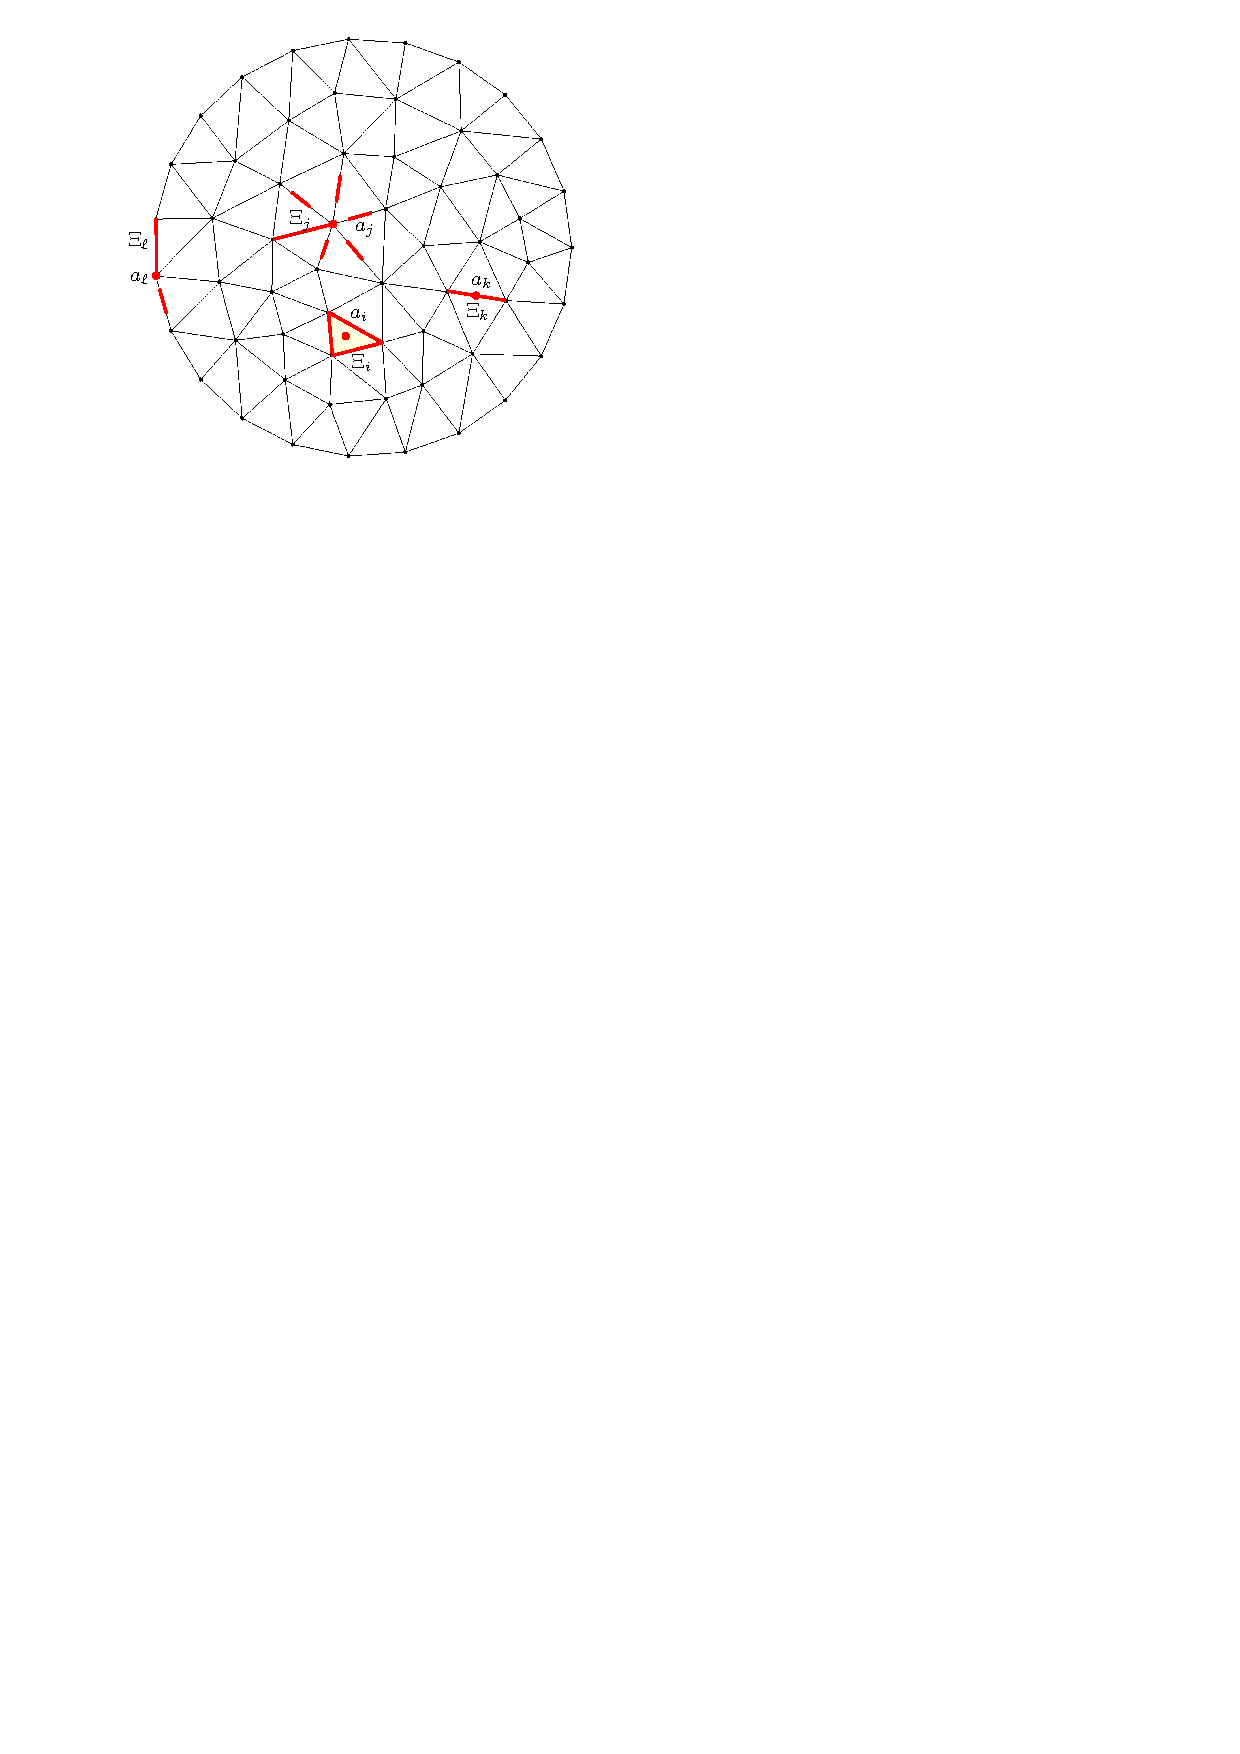
\includegraphics{figures/scott_zhang.pdf}
    \caption{Example choice of the sets $\Xi$ for different types of support points in the Scott-Zhang interpolator. Case $a_i$: support point on the interior of a triangle -- $\Xi_i$ is the triangle itself. Case $a_j$: support point on an internal vertex of the triangulation -- $\Xi_i$ is one of the edges that insist on that vertex. Case $a_k$: support point on the interior of an edge within $\Omega$ -- $\Xi_k$ is the edge itself. Case $a_\ell$: support point on the boundary of the triangulation -- $\Xi_\ell$ is one of the edges that contain $a_\ell$. When multiple choices are possible, we can pick any one (shown as partial red lines in the figure).}
    \label{fig:scott_zhang}
\end{figure}

How do we construct it? Recall that $V_h = \Span\{v_i\}_{i=1}^N$ for some $N$. Let $\{a_1, \dots , a_N\}$ be the Lagrange nodes (support points).
Given a node $a_i$, we associate either a $d$-simplex or a $(d-1)$-simplex $\Xi_i$ to it, as follows (see Figure~\ref{fig:scott_zhang}):
\begin{itemize}
    \item If $a_i \in \mathring{\overline{T}}$ for some $T \in \T_h$, i.e. $a_i$ is in the interior of an element, then $\Xi_i := T$ itself.
    \item If $a_i \in \partial T \setminus \partial \Omega$, i.e. $a_i$ is on some face in the interior of $\Omega$, we choose a face $F$ containing $a_i$ and set $\Xi_i := F$.
    \item If $a_i \in \partial T \cap \partial \Omega$, i.e. $a_i$ is on some face at the boundary, we choose a face $F$ \emph{at the boundary} containing $a_i$ and set $\Xi_i := F$.
\end{itemize}
In the first case, $\Xi_i$ is a $d$-simplex, otherwise it is a $(d-1)$-simplex. Notice that the choice of the face may not be unique, but this will not be relevant. It is only important to choose faces at the boundary for nodes at the boundary, in order for $\SZ$ to preserve homogeneous boundary conditions.

Next, let $n_i$ be the number of nodes belonging to $\Xi_i$ and let $\{v_{i,q}\}_{q=1}^{n_i}$ the restrictions to $\Xi_i$ of the basis functions associated to those support points. Conventionally, we order those functions to have $v_i = v_{i,1}$. Then, for every $q=1,\dots,n_i$, consider the function $\gamma_{i,q} \in \Span\{v_{i,q}\}$ such that
\begin{equation}\label{eqn:sz_def}
    \int_{\Xi_i} \gamma_{i,q} v_{i,r} = \delta_{qr} \quad \forall r=1,\dots,n_i.
\end{equation}
Such a function is unique because of the properties of the $v_{i,r}$ (we have to solve a non-singular linear system). Finally, we define:
\[
\SZ u := \sum_{i=1}^N v_i \int_{\Xi_i} \gamma_{i,1} u = 
\sum_{i=1}^N S^i(u) v_i,
\]
where each linear functional $S^i$ is defined as
\[
S^i(u) := \int_{\Xi_i} \gamma_{i,1} u.
\]
Let us verify that $\SZ$ has indeed the required properties:
\begin{itemize}
    \item If $\gamma$ is the trace operator and $u \in H^1_0(\Omega)$, then $\gamma \SZ u = 0$ by construction.
    \item By the linearity of the $S^i$-s, $\SZ$ is a linear operator. Then, to check if $\SZ u_h = u_h$ for every $u_h \in V_h$, it is sufficient to prove it on a basis of $V_h$. Indeed,
    \[
        \SZ v_j = \sum_{i=1}^N v_i \int_{\Xi_i} \gamma_{i,1} v_j = \sum_{i=1}^N v_i \delta_{ij} = v_j.
    \]
    In particular, the equality
    \[
    \int_{\Xi_i} \gamma_{i,1} v_j = \delta_{ij}
    \]
    follows from \eqref{eqn:sz_def} because, for $j \ne i$, $v_j$ will be either outside $\Span\{v_{i,q}\}$ or equal to $v_{i,r}$ for $r \ne 1$.
\end{itemize}

\begin{remark}
    As we know, the global shape functions $v_i$-s satisfy
    \[
    v^i(v_j) = \delta_{ij}
    \]
    where the $v^i$-s are the global degrees of freedom. We have just seen that the same property holds for the $S^i$-s. Therefore we can see $\SZ$ as a modified Lagrange-type interpolation operator. Remember that the usual Lagrange interpolation is defined by
    \[
    \Pi u = \sum_{i=1}^N v^i(u) v_i.
    \]
\end{remark}

\begin{figure}
    \centering
    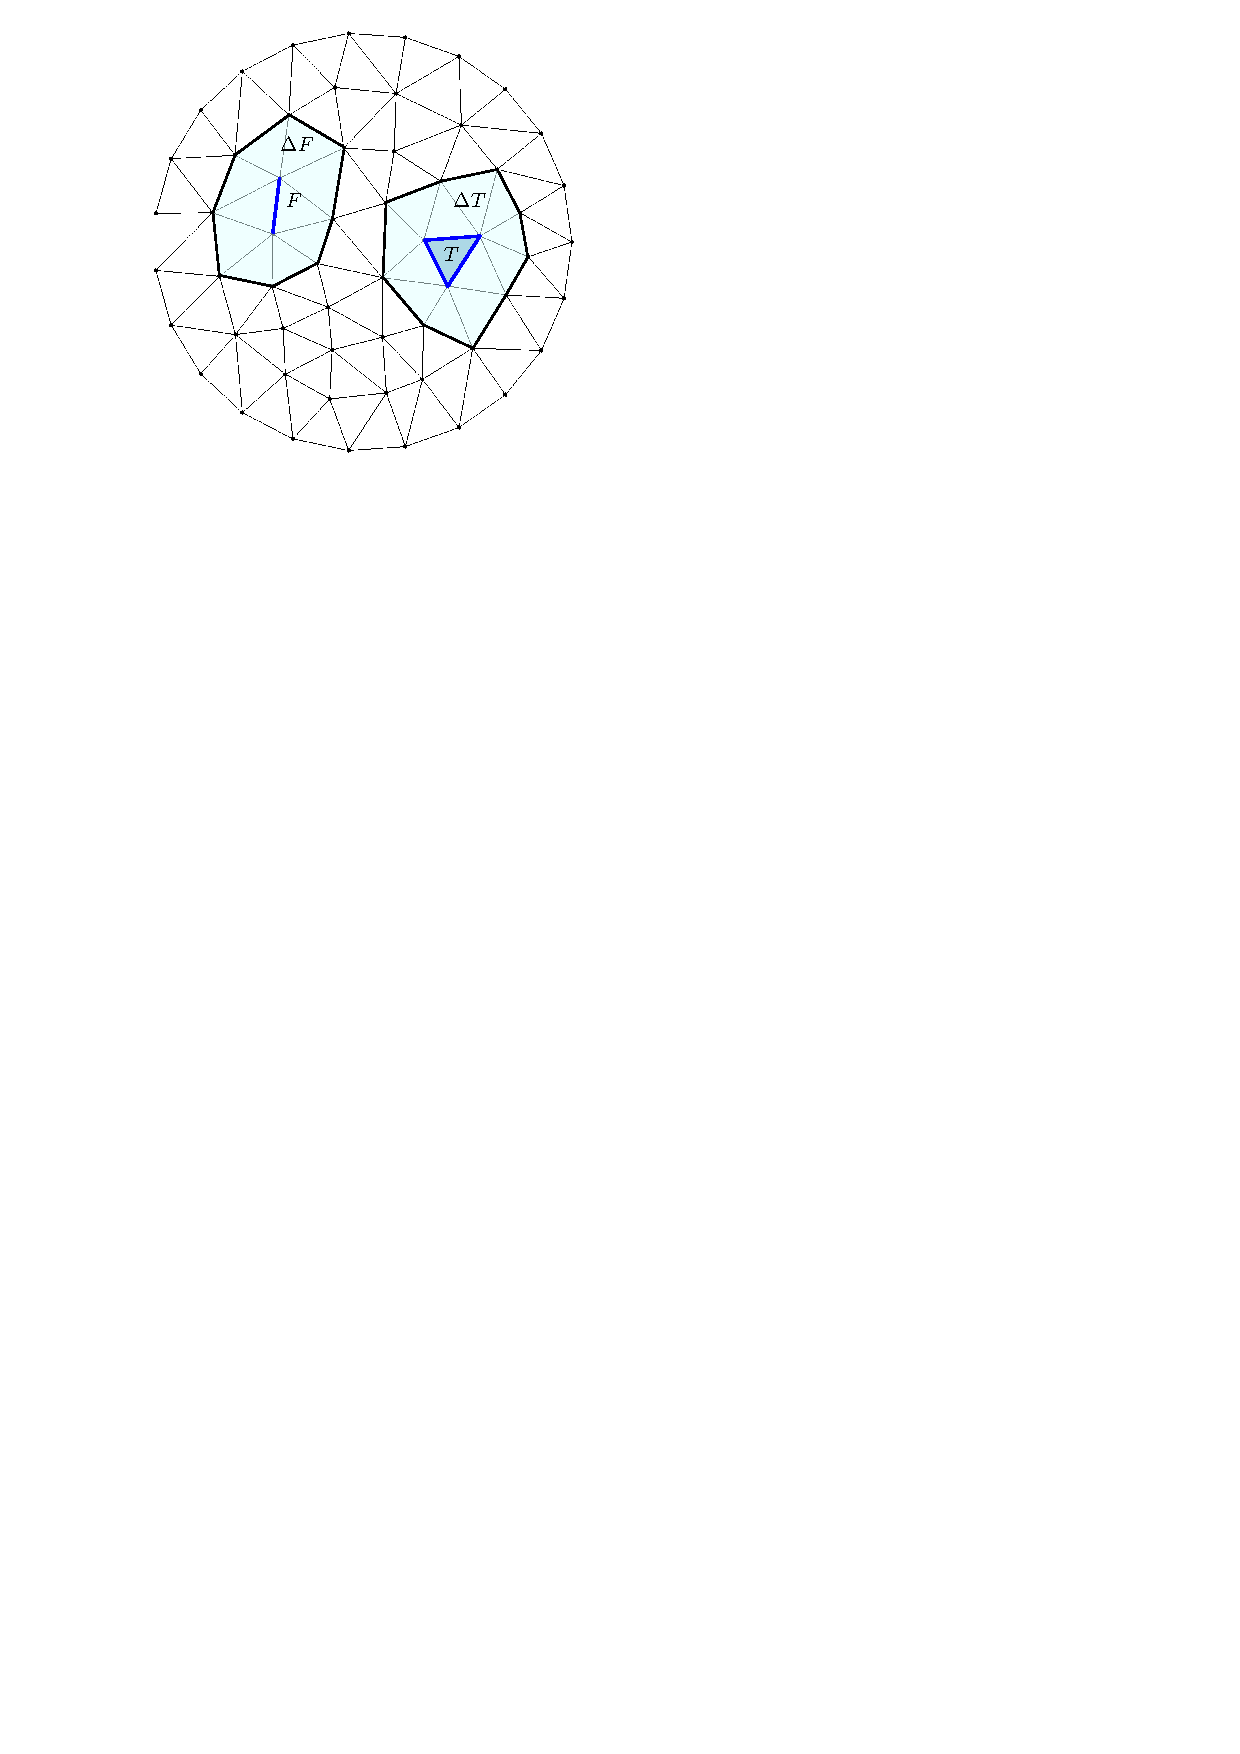
\includegraphics{figures/scott_zhang_patches.pdf}
    \caption{The approximation properties of the Scott-Zhang interpolation operator $\SZ$ are defined in terms of the local patches $\Delta T$ and $\Delta F$. The patch $\Delta T$ is the union of all elements that share at least one vertex with $T$, while the patch $\Delta F$ is the union of all elements that share at least one vertex with $F$.}
    \label{fig:scott_zhang_patches}
\end{figure}

The interpolation properties of $\SZ$ are stated in the following lemma.
\begin{lemma}[Scott-Zhang]
    Let $1\le p < +\infty$ and choose $\ell\ge1$ if $p=1$ or $\ell>\frac{1}{p}$ otherwise. Then the operator $\SZ$ is a projection from $W^{\ell,p}(\Omega)$ to $\P^{k,0}(\Omega)$, with the following properties:
    \begin{enumerate}
        \item Stability: for all $0 \le m \le \min(1,\ell)$,
        \[
        \forall h, \, \forall v \in W^{\ell,p}(\Omega) \quad 
        \norm{\SZ v}_{m,p,\Omega} \lesssim \norm{v}_{\ell,p,\Omega}.
        \]
        In particular, this is true for $m=\ell$.
        \item Approximation on elements: given $0\le m\le \ell\le k+1$,
        \[
        \forall h, \, \forall T \in \T_h, \, \forall v \in W^{\ell,p}(\Delta T) \quad 
        \norm{v- \SZ v}_{m,p,T} \lesssim h_T^{\ell-m} \abs{v}_{\ell,p,\Delta T}.
        \]
        \item Approximation on interfaces: given $m+\frac{1}{p}\le \ell\le k+1$,
        \[
        \forall h, \, \forall F \in \E^i, \, \forall v \in W^{\ell,p}(\Delta F) \quad 
        \norm{v- \SZ v}_{m,p,F} \lesssim h_F^{\ell-m-\frac{1}{p}} \abs{v}_{\ell,p,\Delta F}.
        \]
    \end{enumerate}
    Here $\Delta T$ is the set of elements in $\T_h$ that share at least one vertex with $T$. Analogously, if $F$ is an interface between two elements of $\T_h$, $\Delta F$ is the set of elements in $\T_h$ which share at least one vertex with $F$ (see Figure~\ref{fig:scott_zhang_patches}).
\end{lemma}

\subsection{Orthogonal projections}

Take $V_h = \P^{k,0}(\Omega)$ as in the previous subsection. Since $V_h \subset H^1(\Omega)$, we can consider the following orthogonal projection operators:
\[
    \Pi^0: L^2(\Omega) \to V_h, \qquad
    \Pi^1: H^1(\Omega) \to V_h,
\]
which are, respectively, the projections induced by the scalar products:
\begin{align}
    (u,v)_{0,\Omega} &= \int_\Omega uv, \\
    (u,v)_{1,\Omega} &= \int_\Omega uv + \int_\Omega \nabla u \nabla v.
\end{align}
In practice, $\Pi^0 u$ (respectively $\Pi^1 u$) gives us the closest function to $u$ with respect to the $L^2$ (resp. $H^1$) norm. Moreover,
\begin{align}
    (\Pi^0 u, v)_0 &= (u, v)_0 \quad \forall v \in V_h, \\
    (\Pi^1 u, v)_1 &= (u, v)_1 \quad \forall v \in V_h.
\end{align}
We refer to $\Pi^0$ as the \emph{$L^2$ projection}, to $\Pi^1$ as the \emph{Riesz projection} or \emph{elliptic projection}.

\textbf{------------start of probably wrong part\\}
We look for a way to express these with respect to the basis functions $\{v_i\}$. For simplicity, from now on we will use Einstein's notation. If $u \in L^2(\Omega)$, then $\Pi^0 u$ can be seen as a linear combination of the $v_i$-s:
\[
\Pi^0 u = u^i v_i
\]
where $u^j = v^j(u)$.
\rev{I think this is not true. This would mean that the Lagrange interpolation is an orthogonal projection, which is false in general.}
Set $U^0_i = (u,v_i)_0$. If $M$ is the matrix such that $M_{ij} = (v_j, v_i)_0$, then by linearity
\[
U^0_i = M_{ij} u^j
\]
Now take the inverse matrix of $M$: with this notation, we will call it $M^{ij}$ to stress the fact that
\[
M^{ij} M_{jk} = \delta^i_k.
\]
Then,
\[
\Pi^0 u = M^{ik} (u,v_k)_0 v_i.
\]
\textbf{-------------end of probably wrong part}

\begin{lemma}[stability of orthogonal projections]
    Let $k\ge1$. The following estimates hold:
    \begin{align}
        \forall v \in L^2(\Omega) \quad \norm{\Pi^0 v}_{0,\Omega} &\le \norm{v}_{0,\Omega}, \\
        \forall v \in H^1(\Omega) \quad \norm{\Pi^1 v}_{1,\Omega} &\le \norm{v}_{1,\Omega}.
    \end{align}
    Moreover, if the family of meshes $\{\T_h\}_{h>0}$ is quasi-uniform, then
    \[
        \forall v \in H^1(\Omega) \quad \norm{\Pi^0 v}_{1,\Omega} \lesssim \norm{v}_{1,\Omega}
    \]
    and the constant in the inequality is independent of $h$.
\end{lemma}

\begin{lemma}[approximation of smooth functions]
    Let $k\ge1$ and $1\le l \le k$. Then, for all $v \in H^{l+1}(\Omega)$ we have:
    \begin{align}
        \norm{v - \Pi^0 v}_{0,\Omega} &\lesssim h^{l+1} \abs{v}_{l+1,\Omega}, \\
        \norm{v - \Pi^1 v}_{1,\Omega} &\lesssim h^l \abs{v}_{l+1,\Omega},
    \end{align}
    and the constant is independent of $h$. Moreover, if the family of meshes $\{\T_h\}_{h>0}$ is quasi-uniform, then for all $v \in H^{l+1}(\Omega)$ we have:
    \[
        \norm{v - \Pi^0 v}_{1,\Omega} \lesssim h^l \abs{v}_{l+1,\Omega},
    \]
    again with the constant independent of $h$.
\end{lemma}


\section{A posteriori error analysis}

Turn back to our model Poisson problem:
\[
\begin{cases}
    -\Delta u = f \quad &\text{in } \Omega \\
    u = 0 \quad &\text{on } \partial\Omega
\end{cases}
\]
where the equality $-\Delta u = f$ is taken in $H^{-1}=(H^1_0)'$. So far, we controlled the approximation error \emph{a priori}, i.e. by exploiting theoretical properties of the PDE, like coercivity, to get error estimates. Let us try now a different approach and look for estimates that involve only known quantities, such as the size of the mesh cells, the problem data and the approximate solution $u_h$.

For every element $T$ in the triangulation, we would like to build an estimator $\eta_T = \eta_T(u_h, f)$ such that
\begin{equation}\label{eqn:apost_est1}
    \eta_T^2 \lesssim \abs{u - u_h}_{1,T}^2 \lesssim \eta_T^2,
\end{equation}
locally, and
\begin{equation}\label{eqn:apost_est2}
\sum_{T \in \T_h} \eta_T^2 \lesssim \abs{u - u_h}_{1,\Omega}^2 \lesssim \sum_{T \in \T_h} \eta_T^2,
\end{equation}
globally. In particular, the lower bound of the inequality is referred as \emph{optimality}, the upper one is the \emph{reliability}.
Should such an estimator exist, we could \emph{adapt} the mesh $\T_h$ in order to satisfy two requirements:
\begin{itemize}
    \item Given a tolerance $\texttt{tol}$,
    \[
    \Bigl( \sum_{T \in \T_h} \eta_T^2 \Bigr)^\frac{1}{2} \le \texttt{tol}.
    \]
    \item The error estimator $\eta_T$ is balanced over all the mesh, i.e.
    \[
    \frac{\texttt{tol}}{M} \lesssim \eta_T \lesssim \frac{\texttt{tol}}{M}
    \]
    where $M$ is the number of elements in $\T_h$.
\end{itemize}
Unfortunately, the estimates \eqref{eqn:apost_est1} and \eqref{eqn:apost_est2} are false in general. However, we can prove some weaker -- but still very useful -- results.

In general, we can prove that
\[
\norm{u - u_h}_{1,\Omega}^2 \lesssim \sum_{T \in \T_h} \eta_T^2,
\]
hence global reliability holds. Instead, the lower bound takes an "almost local" form:
\[
\eta_T \lesssim \norm{u-u_h}_{1,\Delta T} + \Pi(h_T,\Delta T,f)
\]
where $\Delta T$ is a patch of elements around $T$ and $\Pi(h_T,\Delta T,f)$ is a perturbation that is either negligible or is asymptotically of the same order as the
error $\norm{u-u_h}_{1,\Delta T}$.

For the Poisson problem, this is the estimator we will be interested in:
\begin{equation}\label{eqn:estimator}
    \eta_T := h_T \norm{f + \Delta u_h}_{0,T}
    + \sum_{F \subset \partial T \setminus \partial\Omega} \frac{1}{2} h_F^{\frac{1}{2}} \norm{\jump{\nabla u_h}}_{0,F}.
\end{equation}
\rev{it seems that the jump function used here is not exactly the same as the jump fn used in discontinuous Galerkin methods, at least if we want to sum also over faces at the boundary. Check this better!}


\subsection{Global reliability}

Assume that the mesh $\T_h$ is shape regular. We have shown in the previous chapters that, if $u$ is regular enough and $A$ is coercive, then
\[
\norm{u-u_h}_{1,\Omega} \lesssim \frac{\norm{A}}{\alpha} \inf_{v_h \in V_h} \norm{u-v_h}
\lesssim \Bigl( \sum_{T \in \T_h} h_T^{2k} \abs{u}_{k+1,T}^2 \Bigr)^{\frac{1}{2}}.
\]
This is an a priori error estimate. In the case $Au = -\Delta u$, the simplest a posteriori estimate we can get is the following:
\begin{equation}\label{eqn:apost_rough}
    \alpha \norm{u-u_h}_{1,\Omega} \lesssim \norm{A(u-u_h)}_{-1,\Omega} = \norm{f+\Delta u_h}_{-1,\Omega}.
\end{equation}
The inequality relies again on coercivity but, leaving room to generalizations, can be shown also if $A$ only satisfies the so called \emph{inf-sup condition}, i.e. the BNB theorem. We will talk about this theorem in chapter~\ref{chap:saddle}.

Inequality~\eqref{eqn:apost_rough} has an issue: it cannot be localized, because the norm in $H^{-1}(\Omega)$ is not local. However, we can work around it following these steps:
\begin{enumerate}
    \item exploit the definition of the $H^{-1}$ norm and the orthogonality of the error;
    \item integrate by parts;
    \item use the properties of Scott-Zhang interpolation.
\end{enumerate}
\boxed{Step 1} For every $v_h \in V_h$ we have
\begin{align}
    \norm{u-u_h}_{1,\Omega} &\lesssim \frac{1}{\alpha} \norm{A(u-u_h)}_{-1,\Omega} \\
    &= \frac{1}{\alpha} \sup_{v \in H^1_0(\Omega)} \frac{\abs{\langle A(u-u_h),v \rangle}}{\norm{v}_{1,\Omega}} \\
    &= \frac{1}{\alpha} \sup_{v \in H^1_0(\Omega)} \frac{\abs{\langle A(u-u_h),v-v_h \rangle}}{\norm{v}_{1,\Omega}}.
\end{align}
\boxed{Step 2} Split the contributions from $u$ and $u_h$ to the integral and remember that $u\in H^1_0(\Omega)$ and $-\Delta u = f$:
\begin{align}
    \langle A(u-u_h),v-v_h \rangle &= \int_\Omega \nabla u \nabla(v-v_h) - \int_\Omega \nabla u_h \nabla(v-v_h) \\
    & = \int_\Omega -\Delta u (v-v_h) - \int_\Omega \nabla u_h \nabla(v-v_h) \\
    & = \sum_{T \in \T_h} \Bigl(\int_T f (v-v_h) - \int_T \nabla u_h \nabla(v-v_h) \Bigr) \\
    & = \sum_{T \in \T_h} \Bigl(\int_T (f + \Delta u_h) (v-v_h) - \int_{\partial T} n \cdot \nabla u_h (v-v_h) \Bigr).
\end{align}
In particular, let us focus on the boundary terms: $v-v_h$ vanishes on $\partial\Omega$, hence the integrals on the boundary involve only interior faces. Globally, each interior face is counted twice, once per side, hence for each cell a jump term shows up with a factor $\frac{1}{2}$. Finally, we take advantage of Cauchy-Schwarz inequality:
\begin{align}
    \langle A(u-u_h),v-v_h \rangle &=
    \sum_{T \in \T_h} \Bigl(\int_T (f + \Delta u_h) (v-v_h) -
    \frac{1}{2} \sum_{F \subset \partial T\setminus\partial\Omega} \int_{F} \jump{\nabla u_h} (v-v_h) \Bigr) \\
    &\lesssim \sum_{T \in \T_h} \Bigl( \norm{f + \Delta u_h}_{0,T} \norm{v-v_h}_{0,T} +
    \frac{1}{2} \sum_{F \subset \partial T\setminus\partial\Omega} \norm{\jump{\nabla u_h}}_{0,F} \norm{v-v_h}_{0,F} \Bigr).
\end{align}
Notice that we have used the continuity of $v-v_h$ across $F$.\\
\boxed{Step 3} The choice of $v_h$ is arbitrary, therefore we can set $v_h = \SZ v$. Then,
\[
\norm{v-\SZ v}_{0,T} \lesssim h_T \abs{v}_{1,\Delta T}
\]
which is the approximation property with $m=0$, $l=1$. Analogously,
\[
\norm{v-\SZ v}_{0,F} \lesssim h_F^{\frac{1}{2}} \abs{v}_{1,\Delta F}.
\]
Wrapping things up, we have shown that
\begin{align}
\abs{\langle A(u-u_h),v-\SZ v \rangle} &\lesssim
\sum_{T \in \T_h} \Bigl( h_T \norm{f + \Delta u_h}_{0,T} +
    \frac{1}{2} \sum_{F \subset \partial T\setminus\partial\Omega} h_F^\frac{1}{2} \norm{\jump{\nabla u_h}}_{0,F} \Bigr) c_T(v) \\
    &= \sum_{T \in \T_h} \eta_T \, c_T(v) \\
    &\le \Bigl( \sum_{T \in \T_h} \eta_T^2 \Bigr)^\frac{1}{2}
    \Bigl( \sum_{T \in \T_h} c_T(v)^2 \Bigr)^\frac{1}{2},
\end{align}
where
\[
c_T(v) = \max \bigl( \abs{v}_{1,\Delta T}, \max_{F \subset \partial T} \abs{v}_{1,\Delta F} \bigr).
\]
\boxed{Step 4} We have to show that
\[
\sum_{T \in \T_h} c_T(v)^2 \le c \norm{v}_{1,\Omega}^2.
\]
for some constant $c$ independent of $h$. Let us exploit the domain additivity of the integral: how many times will $\abs{v}_{1,T}$ show up, at most, in the sum? Let $M$ be the maximum number of times that an element $T$ is part of the neighborhood of another one:
\[
M = \max_{T \in \T_h} \card \Set{T'\in\T_h \text{ s.t. } T \in \Delta T'}.
\]
Similarly, let $N$ be the maximum number of faces an element can be a neighbour of:
\[
N = \max_{T \in \T_h} \card \Set{F\in\E_h \text{ s.t. } T \in \Delta F}.
\]
Clearly, the integers $M$ and $N$ only depend on the shape-regularity of the mesh, and are bounded by a constant independent of $h$, hence we get:
\[
\sum_{T \in \T_h} c_T(v)^2 \le \max(M,N) \norm{v}_{1,\Omega}^2
\le c \norm{v}_{1,\Omega}^2.
\]
This concludes our proof.


\subsection{Quasi-local optimality}

With some effort, we can also show a \emph{quasi-local optimality bound}. Some things need to be defined:
\begin{itemize}
    \item Given a face $F$, we let $D_F$ be the union of elements that share it:
    \[
    D_F := \Set{\mathring{\overline{\bigcup_m \overline{T_m}}} \,\text{ s.t. } \,\overline{T_{m_1}} \cap \overline{T_{m_2}} = F}.
    \]
    In particular, with the assumption that a face can be shared only by two elements, $D_F$ is reduced to the interior part of $\overline{T_{m_1}} \cup \overline{T_{m_1}}$ for some indices $m_1$ and $m_2$.
    \item Given an element $T$, let $D_T$ the union of elements that share a face with $T$:
    \[
    D_T := \Set{\mathring{\overline{\bigcup_m \overline{T_m}}} \,\text{ s.t. }\, \overline{T_m} \cap \overline{T} = F \ne \varnothing, \text{ with }\dim(F)=d-1}.
    \]
\end{itemize}
We shall also introduce \emph{bubble functions}. A bubble function on an element $T$ is a function $b_T$ such that:
\begin{itemize}
    \item $0 \le b_T \le 1$ in $\overline{T}$;
    \item $b_T \in H^1_0(T)$;
    \item $\exists D\subset T$ s.t. $\abs{D}>0$ and $\restr{b_T}{D} \ge \frac{1}{2}$.
\end{itemize}
When $T \subset \R^d$ is a simplex or a hypercube, bubble functions satisfy the following properties, given $\phi \in \P^k(T)$ with $k\ge1$:
\begin{itemize}
    \item $\norm{b_T \phi}_{0,T} \lesssim \norm{\phi}_{0,T} \lesssim \norm{b_T^{\frac{1}{2}} \phi}_{0,T}$;
    \item $\abs{b_T \phi}_{1,T} \lesssim h_T^{-1} \norm{\phi}_{0,T}$ (inverse inequality).
\end{itemize}
\rev{maybe say a word on how this is proved (passing to the finite element, bla bla)}
We want to also introduce bubble functions on faces. These are more complicated, because we would like to \emph{lift} a face, i.e. build an object on $T$ from its face $F$. In order to do this, we consider a \emph{lifting operator}
\[
\RE: \P^k(F) \to \P^k(D_F)
\]
where $\P^k(D_F)$ is considered element-wise.
\rev{tell how this works}

A bubble function on a face $F$ \emph{and} on $D_F$, meaning that it is a bubble function for both $F$ as a $(d-1)$-manifold and for $D_F$ as a $d$-manifold, is a function $b_F$ such that:
\begin{itemize}
    \item $0 \le b_F \le 1$ in $\overline{F}$;
    \item $\restr{b_F}{F} \in H^1_0(F)$ and $b_F \in H^1_0(D_F)$;
    \item $\exists \Tilde{D}_F\subset F$ such that $\abs{\Tilde{D}_F}>0$ and $\restr{b_F}{\Tilde{D}_F} \ge \frac{1}{2}$;
    \item $\exists \Tilde{D}_{D_F}\subset D_F$ such that $\abs{\Tilde{D}_{D_F}}>0$ and $\restr{b_F}{\Tilde{D}_{D_F}} \ge \frac{1}{2}$.
\end{itemize}
Note that $\abs{\Tilde{D}_F}$ is a measure of dimension $d-1$, while $\abs{\Tilde{D}_{D_F}}$ is a measure dimension $d$. Given $\phi \in \P^k(F)$, bubble functions on faces satisfy the following properties:
\begin{itemize}
    \item $\norm{b_F \phi}_{0,F} \lesssim \norm{\phi}_{0,F} \lesssim \norm{b_F^{\frac{1}{2}} \phi}_{0,F}$;
    \item $h_F^\frac{1}{2} \norm{\phi}_{0,F} \lesssim \norm{b_F \RE(\phi)}_{0,D_F} \lesssim h_F^\frac{1}{2} \norm{\phi}_{0,F}$;
    \item $\abs{b_F \RE(\phi)}_{1,D_F} \lesssim h_F^{-\frac{1}{2}} \norm{\phi}_{0,F}$.
\end{itemize}

Bubble functions will come in handy to prove the following result, because using them as weights when integrating by parts will cancel out boundary terms.
\begin{theorem}[local optimality, Verf\"{u}rt 1992-94]
    In the setting above, if $T$ is \emph{shape regular}, i.e. $h_F \sim h_T$, the following inequality holds:
    \[
    \eta_T \lesssim \abs{u - u_h}_{1,D_T} + h_T \inf_{v_h \in V_h} \norm{f - v_h}_{0,D_T}.
    \]
\end{theorem}
\begin{proof}
    We start by estimating the term $\norm{f + \Delta u_h}_{0,T}$ via the triangle inequality:
    \[
    \norm{f + \Delta u_h}_{0,T} \le \norm{f - v_h}_{0,T} + \norm{v_h + \Delta u_h}_{0,T} \qquad \forall v_h \in V_h.
    \]
    Next, consider a bubble function $b_T$ on $T$ and exploit its properties to give an estimate to the second term at the right-hand side:
    \begin{align}
        \norm{v_h + \Delta u_h}_{0,T}^2
        & \lesssim \norm{b_T^{\frac{1}{2}} (v_h + \Delta u_h)}_{0,T}^2 \\
        & = \int_T (v_h + \Delta u_h) b_T (v_h + \Delta u_h) \\
        & = \int_T (v_h -f + \Delta (u_h-u)) b_T (v_h + \Delta u_h) \\
        & = \int_T (v_h -f) b_T (v_h + \Delta u_h) + \int_T \Delta(u_h -u) b_T (v_h + \Delta u_h) \\
        & \lesssim \norm{v_h -f}_{0,T} \norm{b_T (v_h + \Delta u_h)}_{0,T} + \int_T \Delta(u_h -u) b_T (v_h + \Delta u_h) \\
        & \lesssim \norm{v_h -f}_{0,T} \norm{v_h + \Delta u_h}_{0,T} + \int_T \Delta(u_h -u) b_T (v_h + \Delta u_h).
    \end{align}
    In particular, $v_h + \Delta u_h$ is indeed a polynomial on $T$ and we have added $0 = f + \Delta u$ at a certain point. Now integrate by parts: being $b_T \in H^1_0(T)$, we get no boundary terms, hence the chain of inequalities continues:
    \begin{align}
        \norm{v_h + \Delta u_h}_{0,T}^2
        & \lesssim \norm{v_h -f}_{0,T} \norm{v_h + \Delta u_h}_{0,T} - \int_T \nabla(u_h -u) \nabla(b_T (v_h + \Delta u_h)) \\
        & \lesssim \norm{v_h -f}_{0,T} \norm{v_h + \Delta u_h}_{0,T} + \abs{u_h-u}_{1,T} \abs{b_T (v_h + \Delta u_h)}_{1,T} \\
        & \lesssim \norm{v_h -f}_{0,T} \norm{v_h + \Delta u_h}_{0,T} + \abs{u_h-u}_{1,T} \cdot h_T^{-1} \norm{v_h + \Delta u_h}_{0,T} .
    \end{align}
    After canceling $\norm{v_h + \Delta u_h}_{0,T}$ from both sides of the inequality, we get
    \[
        \norm{v_h + \Delta u_h}_{0,T}
        \lesssim \norm{v_h -f}_{0,T} + h_T^{-1} \abs{u_h-u}_{1,T}
    \]
    which implies
    \begin{equation}\label{eqn:verfurt1}
    h_T \norm{f + \Delta u_h}_{0,T}
    \lesssim h_T \norm{f - v_h}_{0,T} + \abs{u_h-u}_{1,T} \qquad \forall v_h \in V_h.        
    \end{equation}

    On to the second term in the error estimator: the idea is to recover $\abs{u_h - u}_{1,T}$ via a bubble function $b_F$ on $F$. We have:
    \begin{align}
        \norm{\jump{\nabla u_h}}_{0,F}^2
        & \lesssim \norm{b_F^{\frac{1}{2}} \jump{\nabla u_h}}_{0,F}^2 \\
        & = \int_F \jump{\nabla u_h} b_F \jump{\nabla u_h} \, dF \\
        & = \int_F \jump{\nabla u_h - \nabla u} b_F \jump{\nabla u_h} \, dF \\
        & = \int_F \jump{\nabla u_h - \nabla u} b_F \RE(\jump{\nabla u_h}) \, dF .
    \end{align}
    In particular, the last two equalities follow from $u$ being the exact solution, hence satisfying $\jump{\nabla u} = 0$ on $F$, and from $\jump{\nabla u_h} = \RE(\jump{\nabla u_h})$ on $F$. To proceed, we use the following remark:
    \begin{remark}
        If $v, z \in H^1(D_F)$, integration by parts implies:
        \begin{align}
            \sum_{T \in D_F} \int_T -\Delta z v
            & = \sum_{T \in D_F} \Bigl(\int_T \nabla z \nabla v - \int_{\partial T} \nabla z \cdot n \, v \Bigr) \\
            & = \int_{D_F} \nabla z \nabla v - \int_F \jump{\nabla z} v - \int_{\partial D_F} \nabla z \cdot n \, v
        \end{align}
        In particular, if also $v \in H^1_0(D_F)$ we obtain:
        \[
        \int_F \jump{\nabla z} v = \int_{D_F} \Delta z v + \int_{D_F} \nabla z \nabla v.
        \]
    \end{remark}
    In our case, the function $v = b_F \RE(\jump{\nabla u_h})$ is indeed in $H^1_0(D_F)$, hence we can continue the chain of inequalities above:
    \begin{align}
        \norm{\jump{\nabla u_h}}_{0,F}^2
        & \lesssim \int_{D_F} (\Delta u_h - \Delta u) b_F \RE(\jump{\nabla u_h}) + \int_{D_F} \nabla (u_h - u) \nabla (b_F \RE(\jump{\nabla u_h}))\\
        & = \int_{D_F} (\Delta u_h + f) b_F \RE(\jump{\nabla u_h}) + \int_{D_F} \nabla (u_h - u) \nabla (b_F \RE(\jump{\nabla u_h})) \\
        & \lesssim \norm{\Delta u_h + f}_{0,D_F} \norm{b_F \RE(\jump{\nabla u_h})}_{0,D_F} + \abs{u_h - u}_{1,D_F} \abs{b_F \RE(\jump{\nabla u_h})}_{1,D_F} \\
        & \lesssim \norm{\Delta u_h + f}_{0,D_F} \cdot h_F^\frac{1}{2} \norm{\jump{\nabla u_h}}_{0,F} + \abs{u_h - u}_{1,D_F} \cdot h_F^{-\frac{1}{2}} \norm{\jump{\nabla u_h}}_{0,F}.
    \end{align}
    As a consequence, simplifying $\norm{\jump{\nabla u_h}}_{0,F}$ from both the sides of the inequality leads to
    \[
    \norm{\jump{\nabla u_h}}_{0,F} \lesssim h_F^\frac{1}{2} \norm{\Delta u_h + f}_{0,D_F} 
    + h_F^{-\frac{1}{2}} \abs{u_h - u}_{1,D_F}
    \]
    and finally
    \begin{equation}\label{eqn:verfurt2}
    h_F^\frac{1}{2} \norm{\jump{\nabla u_h}}_{0,F}
    \lesssim h_F \norm{\Delta u_h + f}_{0,D_F} + \abs{u_h - u}_{1,D_F}.
    \end{equation}
    The conclusion follows immediately grouping inequalities~\eqref{eqn:verfurt1} and~\eqref{eqn:verfurt2} and taking the infimum over $v_h \in V_h$. In particular, summing over $F\subset \partial T$ is the reason why $D_T$ appears in the end.
\end{proof}


\section{Using the error estimator to refine a mesh}

Having a reliable error estimator means that we can impose a certain tolerance to be satisfied:
\[
\abs{u - u_h}_{1,\Omega} \lesssim \Bigl( \sum_T \eta_T^2 \Bigr)^\frac{1}{2} \lesssim \text{tol}.
\]
This way, we can control the error on the solution after having computed the approximation and, eventually, refine the mesh to improve accuracy.

If $\T^i$ is the $i$-th stage of refinement of a triangulation $\T$ and $M^i := \#\T^i$ is its number of elements, one possibility is to require for the following stage $\T^{i+1}$ to satisfy
\[
\eta_T^2 \lesssim \frac{\text{tol}^2}{M^{i+1}} \qquad \forall T \in \T^{i+1}.
\]
\rev{is this someway related to the fixed number algorithm?}

Another way is to use the \emph{bulk chasing algorithm}, also called \emph{D\"{o}rfler} or \emph{fixed fraction} algorithm, or \emph{bulk criterion}. Given $0<\theta<1$, we define the total error at stage $i$
\[
E_{tot} = \Bigl( \sum_{T \in \T^i} \eta_T^2 \Bigr)^\frac{1}{2}.
\]
The aim is to mark for refinement the smallest subset $M \subset \T^i$ such that
\[
\theta E_{tot} \le \Bigl( \sum_{T \in M} \eta_T^2 \Bigr)^\frac{1}{2}
\]
with the following steps:
\begin{enumerate}
    \item Order the elements $T^i_k \in \T^i$ based on the reliability estimator, from the greatest value to the smallest one:
    \[
    \eta_{T^i_k} \le \eta_{T^i_j} \quad \text{when } j \le k.
    \]
    \item Compute $E_{tot}$.
    \item Find $\overline{k}$ such that
    \[
    \Bigl( \sum_{j=1}^{\overline{k}} \eta_{T^i_j}^2 \Bigr)^\frac{1}{2} \ge \theta E_{tot}, \qquad \Bigl( \sum_{j=1}^{\overline{k}-1} \eta_{T^i_j}^2 \Bigr)^\frac{1}{2} < \theta E_{tot}.
    \]
    Then mark for refinement up to element $\overline{k}$.
\end{enumerate}
With an analogous procedure, we can mark another fraction of elements for coarsening, if desired. The result of this process is that the error tends to be distributed "uniformly" over the mesh. In the context of quasi uniform meshes (i.e. $h_{min} \sim h_{max}$) we have
\[
\min_{T \in \T} h_T \lesssim \max_{T \in \T} h_T \lesssim \max_{T \in \T} h_T^{-1}
\lesssim \min_{T \in \T} h_T^{-1},
\]
therefore
\[
\frac{\abs{\Omega}}{M} \sim h_T^d, \quad \text{i.e. } h_T \sim M^{-\frac{1}{d}}.
\]
To give an idea of the impact of a mesh refinement on the global error, let us recall the a priori error estimate~\eqref{ineq:cea_scaling2} we produced in the previous chapter:
\[
\norm{u-u_h}_m \lesssim h^{l-m} \abs{u}_{l} \quad \forall 0\le m \le l-1 \text{ suitable},
\]
with $l \le k+1$, where $k$ is the finite element degree.
\rev{did I say that last thing in the previous chapter? Check}
Then, this implies:
\[
\norm{u-u_h}_m \lesssim M^{-\frac{l-m}{d}} \abs{u}_{l} \quad \forall 0\le m \le l-1 \text{ suitable}.
\]
For example, in the case of a linear FEM approximation ($k=1$) for a Poisson problem on a Lipschitz, convex domain, we have said that this equality holds for $l=2$ and $m=0,1$, because we have also Nitsche's lemma in hand:
\[
\norm{u-u_h}_m \lesssim M^{-\frac{2-m}{d}} \abs{u}_{2}, \quad m=0,1.
\]
This means that the assumption $u \in H^2 \cap H^1_0$ is essential. What happens if $u \not\in H^2$? It can be proven that, if the a posteriori error estimator $\eta$ is equidistributed, i.e. $\eta_k \sim \delta \, \forall k$ (for some value $\delta$), then
\[
\norm{u-u_h}_m \lesssim M^{-\frac{2-m}{d}} \abs{u}_{1}, \quad m=0,1.
\]
Moreover, in that latter context, the hypothesis of quasi-uniformity of the mesh is not needed.

\rev{there's also another inequality in my notes}

Refining the mesh a posteriori implies that, in order to reach a desired level of accuracy, we may need to compute the numerical solution $u_h$ multiple times on progressively refined meshes. Moreover, for time dependent PDEs, further problems arise when dealing with meshes and basis functions that may be different from one time step to another. For the moment, let us stick to stationary problems and conclude this section with some comments and tips on how to use adaptive mesh refinement intelligently:
\begin{itemize}
    \item Calculating the solution multiple times may be worrying in terms of computational time, but needs not to be always. We can put ourselves in the situation where the leading numerical cost is comparable to that of the iteration with the most refined mesh. For example, suppose that each mesh refinement roughly doubles the number of cells and suppose we are using linear elements. If we have $M$ cells at some time, at previous iterations the cells were $\frac{M}{2}$, $\frac{M}{4}$, etc. If we had a perfect solver for the linear system which takes $O(M)$ flops, the total computational effort would be $O(M)+O\bigl(\frac{M}{2}\bigr)+O\bigl(\frac{M}{4}\bigr)+\dots=O(2M)$. To make a comparison with the best possible scenario, a global refinement in 2D quadruplicates the number of cells, hence the total cost would be $O(\frac{4}{3}M)$, which is not too much different.
    Furthermore, when the finite element degree is greater than $1$, this phenomenon is even more evident.
    \item At starting point, i.e. when the numerical solution has not been computed yet, we can assume $u_h=0$, hence
    \[
    \eta_T = h_T \norm{f}_{0,T}.
    \]
    This can be used as a first estimate in order to make the error already equidistributed.
    \item At each refinement step, instead of providing a random guess to start the iterative solver, we can use the solution $u_h$ computed at the previous step, which hopefully will be nearer the exact solution and speed up the convergence. This requires to interpolate that solution to the new mesh, in order to use a vector of the right dimension.
    \item Some solvers such as the conjugate gradient method have a speed-up property: high frequency oscillations do converge very fast (= in a few steps) to the exact ones. Also, those high frequency oscillations carry the largest part of the error. Therefore, at intermediate refinement steps, one could apply just a few iterations of the solver and obtain a crude approximation of the solution, which still will give good indications for what cells need to be refined. Then, after some refinements, the solver can be called with the right tolerance and a full computation of the solution can be done.
    \item In some problems, a lighter version of the estimator $\eta_T$, containing only the jump terms, is used:
    \[
        \tilde{\eta}_T = \sum_{F \subset \partial T} \frac{1}{2} h_F^{\frac{1}{2}} \norm{\jump{\nabla u_h}}_{0,F}.
    \]
    This is known as the \emph{Kelly error estimator}. Kelly, Babu\v{s}ka and others proved in~\cite{kelly83} that it is equivalent to the full estimator for the Laplace equation with constant coefficients.
    \rev{check the reference}
\end{itemize}

\rev{the problem of hanging nodes should be at least mentioned}
